\chapter{Funcionamento da plataforma Drop Flash}
\label{ch:identificador}

\section{Cadastro para o Comerciante}

Para os comerciantes solicitarem entregas pela nossa plataforma é necessário realizar um cadastro diretamente pelo Site.

Ao entrar na plataforma o cliente será direcionado para realizar o login e senha se já for cadastrado já poderá realizar o login, caso não tenha o cadastro basta iniciar no ícone novo cadastro, após a realização do cadastro uma nova janela irá aparecer com vários ícones.

\begin{itemize}
    \item Acompanhar suas entregas;
    \item Solicitar uma nova entrega;
    \item Inserir novos credito para futuras entregas;
    \item Cancelar entrega;
    \item Alterar destino de entrega;
    \item Agendar entrega.
\end{itemize}

Conforme imagem abaixo da tela do Gestor onde o comerciante pode solicitar um novo pedido, acompanhar suas entregas, realizar novos créditos para futuras solicitações de entregas, verificar o saldo de créditos disponíveis, acesso ao suporte e monitorar em tempo real onde esta o entregador ou o drone.\\

\begin{figure} [!ht]
  { \centering
    \caption{Tela inicial do site}
    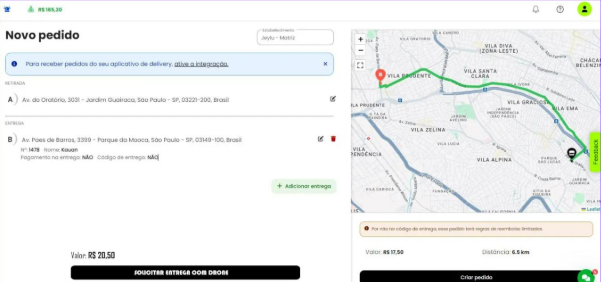
\includegraphics[width=0.5\linewidth]{figuras/funcionamento1.png}
    \label{fig:enter-label}
    \fonte{https://mottu.com.br}
    }
\end{figure}

Para solicitar um novo pedido basta clicar no ícone (novo pedido), o cliente será direcionado para o destino de retirada e local de entregas, pontos adicionais ou não, também será necessário colocar as especificações do produto a ser entregue ao cliente final, tamanho e peso do produto.

Com as informações de local de retirada e destino de entrega, dimensões e peso do produto, como por exemplo:\\

Solicitação de pedido:

\begin{itemize}
    \item Produto farmácia;
    \item Local de retirada e destino de entrega 2km ida e volta;
    \item Tamanho do pacote: 306 x 200 x 190 milímetros;
    \item Peso 1Kg.\\
\end{itemize}

Com essas informações a própria plataforma já vai informar os modelos ideais para esta entrega podendo o cliente optar por Moto ou drone.

\begin{itemize} 
    \item Opção Drone
    \begin{figure} [!ht]
       {\centering
        \caption{DFH - 1}
        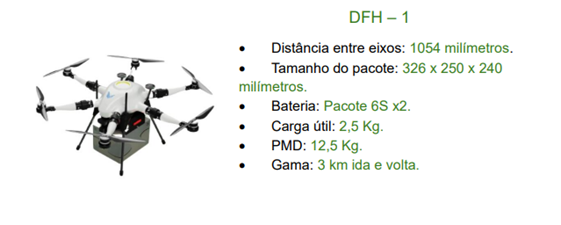
\includegraphics[width=0.9\linewidth]{figuras/drone dfh1.png}
        \label{fig:enter-label}
        \fonte{https://www.speedbird.aero}
        }
    \end{figure}
\\\\\\\\
    
    \item Opção Moto
    \end{itemize}

\begin{figure}[!ht]
    {
    \centering
    \caption{Drop - 110}
    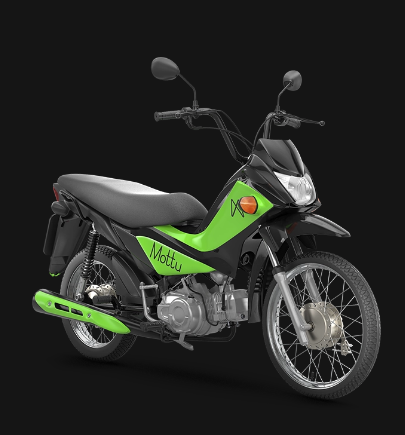
\includegraphics[width=0.5\linewidth]{figuras/Drop110.png}
    \label{fig:enter-label}
    \fonte{https://www.speedbird.aero}
    }
\end{figure}
    


Após finalizar a solicitação de entrega o pedido fica disponível para o entregador, no momento que o entregador aceitar a entrega o cliente poderá acompanhar o pedido em tempo real. O pedido disponível para o entregador, o cliente vai visualizar desta maneira para conseguir acompanhar a sua entrega com mais tranquilidade e transparência.

\begin{figure} [!ht]
   {\centering
    \caption{Acompanhamento do pedido pela plataforma}
    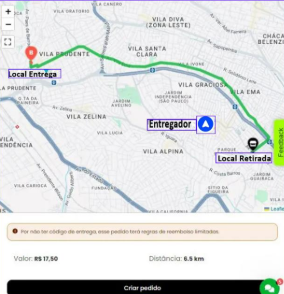
\includegraphics[width=0.4\linewidth]{figuras/pedido.png}
    \label{fig:enter-label}
    \fonte{https://mottu.com.br}
    }
\end{figure}

\section{Cadastro para o entregador}

Para os entregadores ter acesso as entregas pela nossa plataforma é necessários realizar um cadastro diretamente pelo Site ou pelo App disponível nas plataformas da Play Store e App Store. Ao entrar na plataforma o entregador será direcionado para realizar o login e senha se já for cadastrado já poderá realizar o login e realizar as entregas disponíveis, caso não tenha o cadastro basta iniciar no ícone novo cadastro, uma nova janela irá aparecer para o preenchimento do cadastro.

\begin{itemize}
    \item Dados pessoais;
    \item Foto da habilitação;
    \item Foto do rosto para realizar a comparação do documento informado;
    \item Documento do veículo.
\end{itemize}

Após o término do cadastro os dados serão analisados e se tudo 
estiver correto o entregador está apto a utilizar a plataforma. Com o cadastro aprovado o entregador realizará o login e senha, podendo escolher a entrega que estiver disponível na plataforma.\\

O Entregador vai visualizar os pedidos dessa maneira conforme imagem abaixo:

\begin{figure} [!ht]
   {\centering
    \caption{Tela inicial do App para entregadores}
    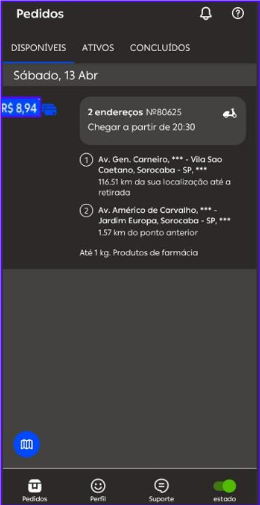
\includegraphics[height=0.5\linewidth]{figuras/app para entregadores.png}
    \label{fig:enter-label}
    \fonte{Borzo Courier}
    }
\end{figure}
\vspace{2cm}
 
Na tela inicial o entregador tem as informações do pedido:
\begin{itemize}
    \item Peso;
    \item Descrição do produto;
    \item Distância entre o entregador está para chegar ao ponto de retirada;
    \item Distância entre o ponto de retirada e entrega do produto.
    \item Valor da entrega;
    \item Hora de retirada e Hora de Entrega.
        \begin{figure} [!ht]
            {\centering
             \caption{Tela inicial do entregador com as informações do pedido}
             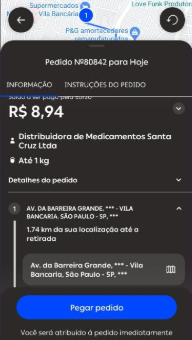
\includegraphics[width=0.5\linewidth]{figuras/infopedido.png}
             \label{fig:enter-label}
             \fonte{Borzo Courier}
            }
        \end{figure}

\end{itemize}

\begin{itemize}
Após o entregador aceitar a corrida na tela vai aparecer a seguinte mensagem:
Você tem certeza que é está rota que deseja?
\end{itemize}

\begin{figure} [!ht]
    {\centering
    \caption{Mensagem de confirmação de rota}
    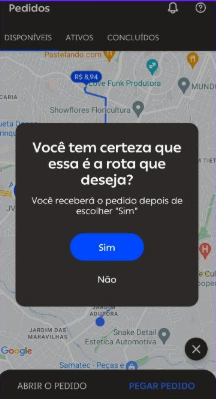
\includegraphics[height=0.5\linewidth]{figuras/mensagementregador.png} 
    \label{fig:enter-label}
    \fonte{Borzo Courier}
    }
\end{figure}

Caso o entregado não aceite a corrida ele é direcionado para a tela de pedidos disponíveis.\\

O entregador aceitando a entrega, ele será direcionado para a tela de rota do pedido e assim o entregador inicia a coleta do pedido para realizar a entrega.

\begin{figure} [!ht]
 {  \centering
    \caption{Tela da rota do pedido}
    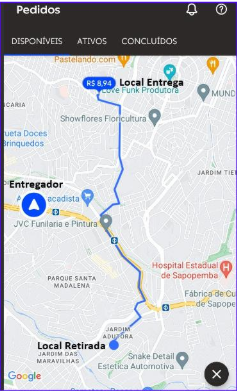
\includegraphics[width=0.3\linewidth]{figuras/rota do entregador.png}
    \label{fig:enter-label}
    \fonte{Borzo Courier}
    }
\end{figure}

Após o entregador finalizar a entrega uma avaliação de satisfação estará disponível para:

\begin{itemize}
    \item Estabelecimento
    \item Entregador
    \item Cliente final
\end{itemize}

A avalição chegará via app conforme imagem abaixo:

\begin{figure} [!ht]
   {\centering
    \caption{Tela de avaliação}
    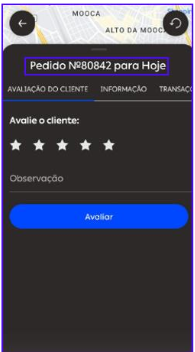
\includegraphics[width=0.5\linewidth]{figuras/avaliacao.png}
    \label{fig:enter-label}
    \fonte{Borzo Courier}
    }
\end{figure}

\begin{figure} [!ht]
   {\centering
    \caption{Tela avaliação finalizado}
    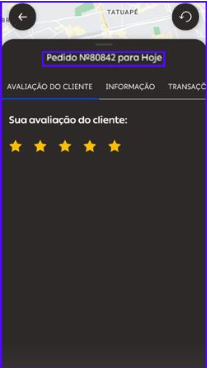
\includegraphics[width=0.5\linewidth]{figuras/image.png}
    \label{fig:enter-label}
    \fonte{Borzo Courier}
    }
\end{figure}

Ao finalizar a entrega e a confirmação do produto solicitado pelo cliente final está tudo certo o valor referente a taxa de entrega já está disponível na conta do entregador que foi informado no momento do cadastro da plataforma.



